\section{Methods}
\label{sec:methods}

The methodology follows a unified pipeline from participant selection to model evaluation and statistical analysis (Figure~\ref{fig:overview}). A primary cohort of 871 participants is selected from ABIDE-I using the available anatomical and functional image-quality ratings. Preprocessed regional time series are obtained from the C-PAC \texttt{filt\_noglobal} derivative using the CC200 atlas and are used to construct three functional-connectivity representations: whole-scan correlation, static tangent-space connectivity, and windowed tangent-space connectivity. Each representation is modelled separately using $\ell_2$-regularised logistic regression, and the resulting probabilities are averaged to form the primary ensemble. Model performance is evaluated using pooled ten-fold cross-validation and leave-one-site-out validation, with regularisation selected within the corresponding training partitions. All data-dependent transformations, including tangent-space references and feature scaling, are estimated from training data before being applied to held-out participants. The resulting out-of-fold predictions form the basis for assessing discrimination, calibration, recalibration, and threshold-based behaviour. Additional analyses examine how participant characteristics, head motion, feature selection, classifier choice, connectivity representation, cohort definition, and other analytical decisions influence the reported results. Functional-connectivity group differences are evaluated separately with nuisance adjustment and motion-matched sensitivity analyses. The linear ensemble members are also examined at the level of functional systems to determine which patterns contribute to classifier scores and how reproducibly these patterns are recovered. Together, these analyses are designed to evaluate not only predictive performance, but also the conditions under which the resulting probabilities, connectivity findings, and model interpretations can be considered reliable.

\begin{figure}[pos=htbp]
\centering
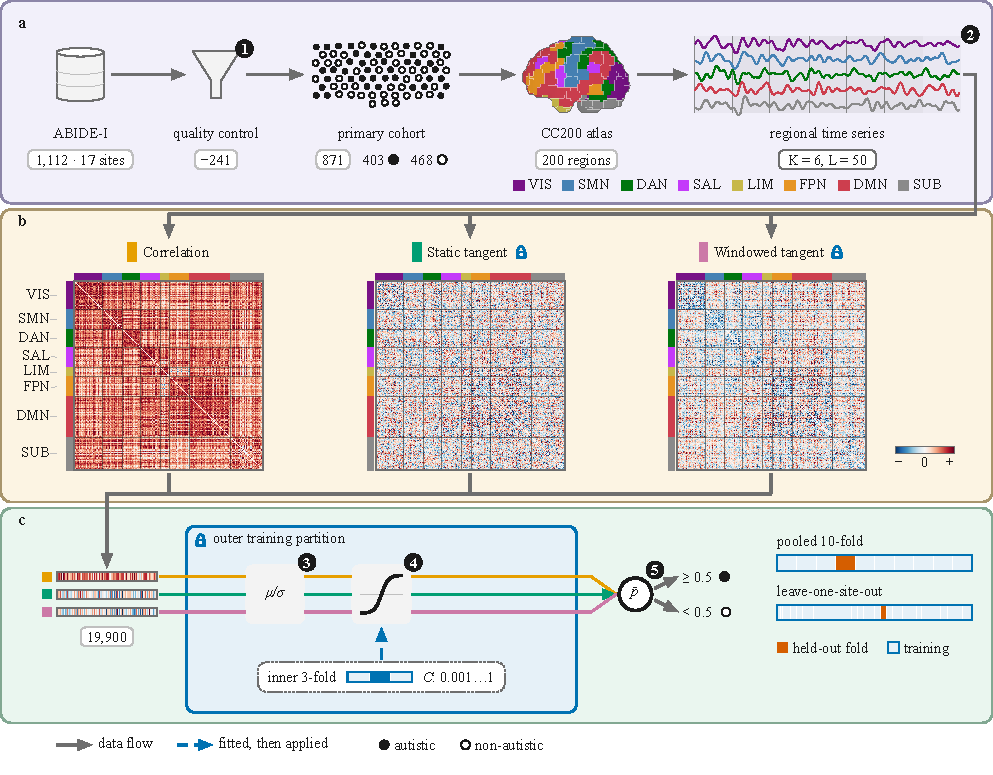
\includegraphics[width=\linewidth,height=0.84\textheight,keepaspectratio]{fig_overview}
\caption{Overview of the primary analysis pipeline. (a) ABIDE-I participants are screened by image-quality control (QC), and CC200 regional time series are extracted from preprocessed rs-fMRI data. Regions are coloured by functional system: VIS, SMN, DAN, SAL, LIM, FPN, DMN, and SUB. (b) Shrinkage-based correlation, static tangent-space connectivity, and windowed tangent-space connectivity are derived, with tangent references estimated from the training partition only. (c) Each representation is vectorised, standardised using training-derived statistics, and classified by $\ell_2$-regularised logistic regression with inner three-fold CV. Model probabilities are averaged for the final ensemble, which is evaluated using pooled ten-fold and LOSO CV. Circled numbers mark \ding{202}~QC, \ding{203}~time series and windows, \ding{204}~scaling, \ding{205}~logistic regression with tuning, and \ding{206}~probability averaging at the 0.5 threshold. Locked blue boxes indicate training-only estimates; grey arrows show data flow, and dashed blue arrows show fitted quantities applied unchanged.}

\label{fig:overview}
\end{figure}

The Methods are organised into ten subsections that follow the analysis pipeline. Section~\ref{subsec:study-design-cohort} describes the study design, data, cohorts, phenotypic variables, atlas, and scan-quality characteristics. Sections~\ref{subsec:connectivity-representations}--\ref{subsec:interpretation} define the connectivity representations, prediction model, validation strategy, probability-based analyses, and interpretation of the linear models. Planned comparisons and exploratory group-contrast analyses are described in Sections~\ref{subsec:planned-comparisons} and~\ref{subsec:group-differences}, followed by the statistical analysis in Section~\ref{subsec:statistical-analysis}. Reproducibility and the scope of the resulting estimates are addressed in Section~\ref{subsec:reproducibility-scope}.


\subsection{Study design and cohort}
\label{subsec:study-design-cohort}

This subsection defines the study question, the data, and the participant cohorts on which
the analyses are based. These definitions are given first, because all representations,
models, and comparisons are based on these data and cohorts. The study design is
described in Section~\ref{subsubsec:study-design}, and the data source and preprocessing in
Section~\ref{subsubsec:data-preprocessing}. The primary cohort is then defined in
Section~\ref{subsubsec:cohorts}, and the wider QC cohort in Section~\ref{subsubsec:cohorts}.
Next, the phenotypic variables and the handling of missing values are specified in
Section~\ref{subsubsec:phenotypic-variables}. The atlas and the signal-quality procedure are described in
Section~\ref{subsubsec:atlas-signal-quality}. Finally, the treatment of differences in scan length is described
in Section~\ref{subsubsec:scan-length}.

\subsubsection{Study design}
\label{subsubsec:study-design}

Clinical diagnosis of ASD combines direct observation,
developmental history, and professional judgement. In this study, ASD status is defined by
the diagnostic labels provided in ABIDE-I, while
rs-fMRI is used to characterise
large-scale functional connectivity in autistic and non-autistic participants. The ASD classification target is derived directly from the ABIDE-I diagnostic labels. Participants with \texttt{DX\_GROUP = 1} are coded as autistic, whereas those with
\texttt{DX\_GROUP = 2} are coded as non-autistic. The primary analysis therefore evaluates
how well the imaging-based models distinguish autistic from non-autistic participants within
the ABIDE-I research cohort.

Discrimination is evaluated primarily using participant-pooled out-of-fold AUROC under pooled ten-fold and
LOSO validation. For each participant, the prediction used for evaluation is
generated by a model fitted without that participant's held-out data, and predictions from
all held-out folds are subsequently combined to calculate the overall AUROC. AUROC is used
as the primary discrimination measure because it assesses the ranking of autistic and
non-autistic participants across prediction scores without requiring a fixed classification
threshold. In pooled ten-fold validation, participants from all sites are distributed across ten folds,
with each fold held out once, providing an estimate of generalisation within the combined
ABIDE-I multisite cohort. LOSO validation instead holds out all participants
associated with one site label at a time, providing a more stringent assessment of
generalisation to an ABIDE-I site that is absent from model training.

The primary prediction model is defined as an equal-weight ensemble of three connectivity representations. Six comparative analyses and two ensemble-level analyses are used to examine the main methodological questions of the study. In four comparative analyses, discrimination across cognitive-ability groups, the persistence of functional-connectivity differences after within-site matching for head motion, the effect of feature-selection scope and granularity, and the performance of different classifier families under the same representation and validation procedure are assessed. In the remaining two, symptom associations and the windowed connectivity description are examined. Classifier-score associations are assessed both across the full cohort and within autistic participants. For windowed connectivity, the same covariance shrinkage is applied to the whole-scan description so that regularisation is matched between the two representations. The ensemble itself is then examined through probability calibration and score attribution. Ensemble probabilities are assessed and recalibrated within the training partitions when systematic offset is identified, and the ensemble score is attributed to functional-system pairs whose reproducibility is tested against a permutation reference. The cognitive-subgroup, head-motion matching, feature-selection, and classifier-comparison procedures are integrated with the validation design in Section~\ref{subsubsec:outer-validation}.


\subsubsection{Data source and preprocessing}
\label{subsubsec:data-preprocessing}

Data are obtained from ABIDE-I, a multi-site research dataset that combines rs-fMRI, anatomical magnetic resonance imaging, and phenotypic information from 1,112 participants across 17 acquisition sites \citep{DiMartinoetal2014}. The phenotypic records provide diagnostic status together with demographic and cognitive measures, including age, sex, full-scale IQ, verbal IQ, performance IQ, handedness, and acquisition site. These variables are retained to characterise the study population and to support the subgroup and covariate analyses described later. After the QC procedure described in Section~\ref{subsubsec:cohorts}, the primary cohort contains 871 participants, including 403 autistic and 468 non-autistic participants. The cohort includes 727 male and 144 female participants and spans 6.5--58 years of age, with a mean age of 16.9 years (standard deviation [SD] 7.6). Mean full-scale IQ is 105.8 in the autistic group and 111.1 in the non-autistic group. Because ABIDE-I combines data acquired independently at multiple centres, heterogeneity remains across sites in scanner hardware, acquisition protocols, scan duration, participant composition, and image quality \citep{Abrahametal2017}. Image quality is therefore considered explicitly during cohort selection using the anatomical and functional quality ratings provided with the release. Preprocessed imaging outputs are obtained from the Preprocessed Connectomes Project \citep{Craddocketal2013}, which provides ABIDE-I data processed through standardised workflows and thereby supports consistent preprocessing across participants from different acquisition sites. The use of these publicly released derivatives also improves reproducibility by fixing the imaging inputs and preprocessing choices. The present study uses outputs generated with C-PAC, specifically the \texttt{filt\_noglobal} processing strategy.

Within the selected C-PAC workflow, temporal and spatial sources of unwanted variation are addressed before functional connectivity is estimated. Slice-acquisition timing differences are corrected, successive functional volumes are realigned to reduce motion-related displacement, non-brain tissue is removed, signal intensities are normalised, and the functional images are aligned with the corresponding anatomical images. Additional variation associated with head motion and non-neural signals is reduced through nuisance regression using a 24-parameter motion model, five CompCor components derived from white-matter and cerebrospinal-fluid signals, and linear and quadratic temporal trends. This processing reduces contributions from residual head motion, physiological noise, and slow signal drift before connectivity is calculated. The resulting signals are then band-pass filtered between 0.01 and 0.10~Hz to retain the low-frequency fluctuations used for resting-state functional-connectivity analysis, while global signal regression is not applied under the selected \texttt{filt\_noglobal} strategy \citep{Craddocketal2013}. Following preprocessing, the functional data are reduced from voxel-level images to atlas-defined regional time series. For the primary analysis, the CC200 atlas divides the brain into 200 functionally defined regions, and the signal within each region is summarised across the scan to produce one time series per region and participant. These 200 regional time series form the common imaging input from which the correlation, static tangent-space, and windowed tangent-space connectivity representations are constructed. Although the common C-PAC workflow reduces variation caused by inconsistent preprocessing procedures, heterogeneity arising from acquisition conditions and participant composition remains part of the ABIDE-I multisite setting. These remaining sources of variation are addressed through QC-based cohort selection, site-aware validation, nuisance adjustment, and the sensitivity analyses described in the following sections.

\subsubsection{Primary and wider quality-control cohorts}
\label{subsubsec:cohorts}

The analysis cohorts are defined using the anatomical and functional image-quality ratings
provided with ABIDE-I. These ratings identify whether the available scans are suitable for
analysis and are accompanied by annotations for issues such as excessive head motion,
unsuccessful skull stripping, incomplete or distorted anatomical coverage, preprocessing
failure, image noise, missing imaging modalities, and regional signal dropout. For the
primary cohort, a participant is retained only when the required assessment from all three
raters is satisfied: rater~1 is required to mark the scan as acceptable; rater~2 is required to rate both the
anatomical and functional images as acceptable or borderline; and rater~3 is required to rate both
images as acceptable. Applying this criterion excludes 241 of the 1,112 ABIDE-I records.
Because the quality annotations sometimes overlap, an excluded scan is potentially associated with more
than one recorded issue. The resulting primary cohort contains 871 participants, including
403 autistic and 468 non-autistic participants. It comprises 727 male and 144 female
participants, with ages ranging from 6.5 to 58 years (mean 16.9 years; median 14.8 years).
Cohort membership is fixed before the primary analyses, and participant identifiers are
cross-checked against the phenotypic records to ensure that the same participants are used
throughout the prediction pipeline. The cohort-selection procedure and subsequent
time-series extraction are summarised in Figure~\ref{fig:overview}a.

Participant characteristics by diagnostic group are reported in
Table~\ref{tab:participants}. Welch's $t$-test is used to compare age and the three IQ measures---full-scale, verbal, and performance---between the
autistic and non-autistic groups, allowing for unequal group variances. Mean FD, defined in Section~\ref{subsubsec:phenotypic-variables}, is examined using both Welch's
$t$-test and the Mann--Whitney $U$ test. The former compares group means, whereas the latter
provides a rank-based comparison that is less sensitive to the right-skewed FD
distribution. Scan length is compared using the Mann--Whitney $U$ test, and sex
distributions are compared using the $\chi^2$ test with Yates' continuity correction.
Because cognitive ability and head motion potentially influence subsequent results, their effects
are examined separately in the cognitive-subgroup analysis of
Section~\ref{par:cognitive-sex-subgroups} and the motion-matched group-contrast analysis of
Section~\ref{subsubsec:system-motion-regional}.

A wider QC cohort is additionally defined to test whether the findings depend
on the more restrictive primary inclusion rule and to support comparison with previous ABIDE-I
studies. For this cohort, eligibility requires an acceptable functional-image rating from
rater~3, without applying the full three-rater criterion used for the primary cohort. This
definition identifies 1,035 eligible participants in the phenotypic records, of whom 1,032
have regional time series available for analysis. The 1,035-participant eligibility count
matches the cohort definition reported by \citet{Heinsfeldetal2018},
\citet{Eslamietal2019}, and \citet{AlmuqhimSaeed2021}. The wider cohort is therefore used
as a cohort-definition sensitivity analysis, allowing the primary results to be assessed
under a less restrictive QC rule while also providing a direct basis for
comparison with these previous reports. The participants of the wider cohort that the primary rule excludes are compared with the primary cohort on mean FD (Mann--Whitney U test), on the proportion of autistic participants (Fisher's exact test), and on the proportion with at least one recorded rater note.

\begin{table}[t]
\centering
\caption{Participant characteristics in the primary cohort (871 participants; 20 site labels from 17 acquisition sites). Values are mean (SD) or median [IQR]; available sample sizes are given in brackets when below the group total.}
\label{tab:participants}
\small
\begin{tabular}{@{}>{\raggedright\arraybackslash}p{0.36\linewidth}ccc@{}}
\toprule
Characteristic & Autistic (n = 403) & Non-autistic (n = 468) & p \\
\midrule
Age, years & 17.07 (7.96) & 16.84 (7.24) & 0.66 \\
Female, n (\%) & 54 (13.4) & 90 (19.2) & 0.027 \\
Full-scale IQ & 105.79 (17.06) [376] & 111.09 (12.08) [435] & $6.2\times10^{-7}$ \\
Verbal IQ & 104.89 (18.10) [342] & 111.57 (13.07) [379] & $2.8\times10^{-8}$ \\
Performance IQ & 105.69 (17.26) [344] & 107.91 (13.05) [391] & 0.052 \\
Mean FD (Section~\ref{subsubsec:phenotypic-variables}), mm & 0.126 (0.143) & 0.094 (0.082) & $8.2\times10^{-5}$ \\
Mean FD (Section~\ref{subsubsec:phenotypic-variables}), mm, median [IQR] & 0.088 [0.057, 0.144] & 0.068 [0.045, 0.109] & $8.9\times10^{-7}$ \\
Volumes per scan, median [range] & 176 [78, 316] & 176 [78, 316] & 0.77 \\
\bottomrule
\end{tabular}

\vspace{4pt}
\begin{minipage}{\linewidth}\footnotesize
p-values are from Welch's t-test for rows summarised by mean (SD), the Mann--Whitney U
test for rows summarised by median, and the $\chi^2$ test with Yates' continuity
correction for sex.
\end{minipage}
\end{table}

\subsubsection{Phenotypic variables}
\label{subsubsec:phenotypic-variables}

Phenotypic information is linked to each participant through the ABIDE-I identifiers and
includes age, sex, full-scale IQ, verbal IQ, performance IQ, handedness, and acquisition
site. These variables are used to characterise the cohort and to support the secondary,
subgroup, and nuisance-adjustment analyses described later. The primary ensemble itself is
restricted to imaging-derived connectivity features, so demographic and cognitive variables
do not contribute directly to its predictions. A separate phenotype model, described in
Section~\ref{par:phenotype-model}, instead uses age, sex, the three IQ measures, and handedness to
evaluate discrimination from non-imaging information. Acquisition site is retained for
site-based validation, nuisance adjustment, and sensitivity analyses. Head motion is represented separately by mean FD, obtained from
the \texttt{func\_mean\_fd} mean-FD quality metric provided with the preprocessed release. This
measure follows Jenkinson's formulation and is calculated from the rigid-body realignment
parameters between successive functional volumes, with rotational components converted to
millimetres using an 80-mm head radius. The resulting mean FD
provides a single scan-level summary of head motion for each participant and is used in the
participant-characteristic comparisons and the subsequent motion-adjusted and
motion-matched analyses.

Missing phenotypic entries are identified before analysis, including values recorded as
\texttt{-9999} or left blank. When phenotypic variables are used in predictive or
harmonisation models, missing continuous values are replaced by the median calculated from
the corresponding outer training partition. This prevents information from held-out
participants from entering preprocessing. The same rule is used for the secondary
phenotype model in Section~\ref{par:phenotype-model} and for age in the ComBat analysis of
Section~\ref{par:combat-harmonisation}. In the ComBat model, sex is coded as 0 for male and 1 for female.
No age or sex values are missing in the primary cohort. For analyses fitted directly to a complete analysis cohort, required missing covariates are
median-imputed from that cohort. This applies to the nuisance-adjustment procedures in
Sections~\ref{par:selection-scope} and~\ref{subsubsec:connection-adjustment}, as well as to the preparation for motion
matching in Section~\ref{subsubsec:system-motion-regional}. In contrast, no imputation is applied in the
symptom-association, cognitive-subgroup, instrument-concordance, component--symptom, or
participant-characteristic analyses. Participants with missing values are excluded only
from the analysis that requires the corresponding variable.

\subsubsection{Atlas and signal quality}
\label{subsubsec:atlas-signal-quality}

The primary analyses use the CC200 functional parcellation~\citep{Craddocketal2012}. All 200 regions are retained for prediction, yielding 19,900 unique pairwise connectivity features. A separate signal-quality check is applied before the group difference analyses because Pearson correlation cannot be computed for a region with no temporal variation. First, any region with a temporal SD of zero in more than 1\% of the 1,032 available CC200 time-series files is removed; four regions meet this criterion. Participants in the primary cohort are then excluded from the group-contrast analysis if any of the remaining regions contains a constant signal. This produces a group-contrast cohort of 863 participants and 196 regions, corresponding to 19,110 unique connections. To support system-level interpretation, each CC200 region is also assigned an anatomical label and a functional-system label. Yeo's seven cortical systems are mapped onto the CC200 space using nearest-neighbour interpolation~\citep{Yeoetal2011}, preserving a single system label for each voxel. Each region is assigned to the system with the greatest spatial overlap when that system covers more than 20\% of the region; regions that do not meet this threshold are assigned to a subcortical/cerebellar category. This procedure yields eight functional-system classes and 36 unique within- and between-system combinations, which are used to summarise connection-level group effects at the system level.

\subsubsection{Scan length}
\label{subsubsec:scan-length}

Scan length is considered explicitly in the dynamic-connectivity analyses because the number of available volumes differs substantially across participants and sites. In the primary cohort, scans contain between 78 and 316 volumes, with scan duration varying systematically by acquisition site. To keep the dynamic representations comparable, each participant contributes the same number of temporal windows regardless of total scan length. This prevents participants with longer scans from contributing more window-level estimates than those with shorter scans. Window length and temporal change are expressed in volumes rather than seconds because a harmonised repetition-time field is not available across the analysis files.

\subsection{Connectivity representations}
\label{subsec:connectivity-representations}

This subsection describes how each participant's regional rs-fMRI time series are
transformed into the three connectivity representations used by the primary ensemble:
shrinkage correlation, static tangent-space connectivity, and windowed tangent-space
connectivity. The first two describe connectivity over the full scan, whereas the third
summarises connectivity estimated from shorter temporal windows. Each representation is
converted into a 19,900 dimensional feature vector for the 200-region CC200 atlas and is
processed independently before classification. The corresponding feature construction,
covariance estimation, tangent-space projection, additional shrinkage, and windowing
procedures are detailed in Sections~\ref{subsubsec:connectivity-features}--\ref{subsubsec:windowed-representation}.

Figure~\ref{fig:representation} summarises this transformation. Whole-scan and window-level
covariance matrices are first estimated using Ledoit--Wolf shrinkage. Static tangent
connectivity is obtained by projecting the whole-scan covariance relative to a Riemannian
reference estimated from the corresponding training partition, while shrinkage correlation
is derived directly from the covariance estimate. For the windowed representation, each
scan is divided into six windows of 50 volumes, and the window covariances receive an
additional isotropic shrinkage of $r=0.15$ before projection to a training-derived dynamic
reference. The resulting window tangent matrices are averaged to form the mean windowed
tangent representation. All training-dependent reference matrices are re-estimated within
each outer fold and then applied unchanged to held-out participants.

\begin{figure}[pos=tbp]
\centering
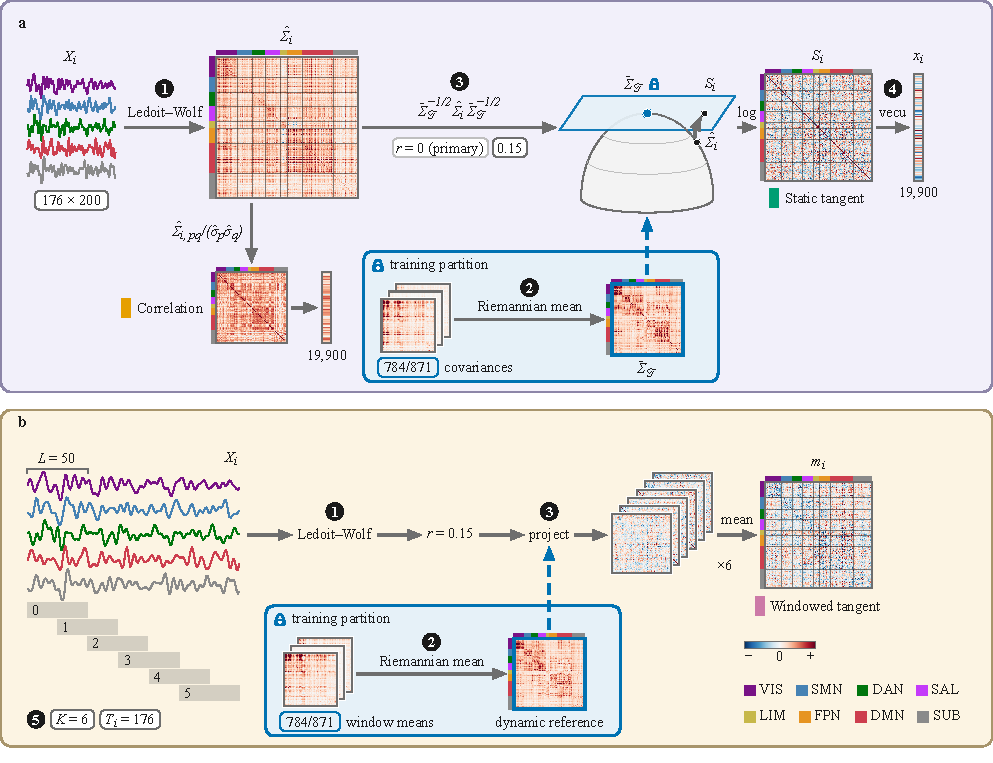
\includegraphics[width=\linewidth]{fig_representation}
\caption{Construction of the connectivity representations for one example participant. (a) \ding{202}~Ledoit--Wolf covariance, \ding{203}~training-only Riemannian reference, \ding{204}~whitening and matrix logarithm, and \ding{205}~vectorisation. A shrinkage-correlation branch is also shown, with additional shrinkage set to $r=0$ in the primary static model and $r=0.15$ in the shrinkage-matched control. (b) \ding{206}~Six windows of 50 volumes are each processed through steps \ding{202}--\ding{204} using a dynamic reference, with additional shrinkage of $r=0.15$ applied before projection, and are then averaged. Locked blue boxes indicate quantities estimated from the training partition only; 784/871 denotes the number of training covariances in a typical outer partition of pooled ten-fold validation.}
\label{fig:representation}
\end{figure}
\subsubsection{Functional-connectivity features}
\label{subsubsec:connectivity-features}

Functional-connectivity features are derived from the regional rs-fMRI time series of each
participant. Each CC200 region is represented by a blood-oxygen-level-dependent signal
recorded across the scan, and connectivity is estimated from the statistical relationship
between pairs of these regional signals. With 200 regions, this produces 19,900 unique
pairwise connectivity features for each participant. Three representations of these
connections are used in the primary ensemble: shrinkage correlation, static tangent-space
connectivity, and mean windowed tangent-space connectivity. The static tangent
representation summarises connectivity across the full scan, whereas the windowed
representation captures the average connectivity pattern across shorter temporal segments.
These three representations are illustrated for one participant in
Figure~\ref{fig:overview}b. Each representation is constructed and standardised separately
so that its fitted reference and scaling parameters remain specific to that representation.

\subsubsection{Shrinkage-correlation features}
\label{subsubsec:shrinkage-correlation}

Shrinkage-correlation features are derived from each participant's Ledoit--Wolf covariance
estimate, defined in Section~\ref{subsubsec:covariance-estimation}. This estimate provides a regularised
description of how the regional signals vary together and is converted to a correlation
matrix by normalising each covariance by the SDs of the corresponding
region pair. The resulting coefficients therefore describe pairwise coupling on a common
scale, independent of regional signal variance. The strict upper triangle of the
correlation matrix is then vectorised into a single feature vector, while the diagonal is
omitted because all self-correlations equal one. This produces 19,900 correlation features
for the CC200 atlas. The same outer-fold partitions are used for this representation and
the two tangent-space representations, ensuring that all three ensemble members are
trained and evaluated on identical participant splits.

\subsubsection{Whole-scan covariance estimation}
\label{subsubsec:covariance-estimation}

Whole-scan covariance is estimated for each participant from all volumes of the regional
time series. For this purpose, $X_i \in \mathbb{R}^{T_i \times P}$ denotes the regional
time series for participant $i$, where $T_i$ is the number of volumes and $P$ is the
number of regions. The covariance is then estimated with Ledoit--Wolf shrinkage
\citep{LedoitWolf2004}, as given in Equation~\eqref{eq:ledoit-wolf-covariance}. In this estimator, the
covariance is a weighted average of the sample covariance and a scaled identity matrix:
\begin{equation}
\widehat{\Sigma}_i
=
(1-\rho_i)\widehat{S}_i
+
\rho_i \widehat{\mu}_i I_P,
\qquad
\widehat{\mu}_i
=
\frac{\operatorname{tr}(\widehat{S}_i)}{P}.
\label{eq:ledoit-wolf-covariance}
\end{equation}

In Equation~\eqref{eq:ledoit-wolf-covariance}, $\widehat{S}_i$ is the sample covariance, $I_P$ is the identity
matrix, and $\widehat{\mu}_i$ is the average of the regional variances. The shrinkage
weight $\rho_i$ is, in turn, selected by the Ledoit--Wolf estimator. Shrinkage is used
because the number of regions is large relative to the number of volumes, which makes the
sample covariance alone an unstable estimate.

\subsubsection{Tangent-space projection}
\label{subsubsec:tangent-projection}

Tangent-space projection converts each covariance matrix into a representation suitable for 
used directly by suitable for direct use bystandard linear classifiers. Because covariance matrices have a
non-Euclidean structure, they are projected relative to a reference matrix estimated from
the training data. This produces a locally linear feature space while preserving the
geometry of the original covariance matrices. The projection process is illustrated in
Figure~\ref{fig:representation}a.

The reference matrix is estimated separately for each outer fold as the affine-invariant
Riemannian mean of the training covariances \citep{Varoquauxetal2010,Dadietal2019}. As
given in Equation~\eqref{eq:riemannian-mean}, this mean is the positive-definite matrix $R$ with the
smallest summed squared distance to the training covariances:
\begin{equation}
\overline{\Sigma}_{\mathrm{T}}
=
\arg\min_{R \succ 0}
\sum_{i \in \mathrm{T}}
\left\|
\log\!\left(R^{-1/2}\widehat{\Sigma}_iR^{-1/2}\right)
\right\|_F^2.
\label{eq:riemannian-mean}
\end{equation}

In Equation~\eqref{eq:riemannian-mean}, $\mathrm{T}$ denotes the training set, and the Frobenius norm is used to quantify the affine-invariant distance between the reference matrix $R$ and each training covariance. The Riemannian mean is therefore adopted as the reference because it respects the geometry of the covariance space. It is estimated by fixed-point iteration with at most ten updates. Matrix logarithms and inverse square roots are computed by symmetric eigendecomposition, with eigenvalues clamped at $10^{-6}$ to maintain numerical stability.

Training and held-out covariances are then projected into the tangent space with the
training reference. As shown in Equation~\eqref{eq:tangent-projection}, each covariance is first multiplied
on both sides by the inverse square root of the reference. The matrix logarithm of this
product then gives the projected matrix $S_i$:
\begin{equation}
S_i
=
\log\!\left(
\overline{\Sigma}_{\mathrm{T}}^{-1/2}
\widehat{\Sigma}_i
\overline{\Sigma}_{\mathrm{T}}^{-1/2}
\right).
\label{eq:tangent-projection}
\end{equation}

The projected matrix in Equation~\eqref{eq:tangent-projection} is then vectorised by retaining only its
off-diagonal upper triangle, as given in Equation~\eqref{eq:vectorisation}. Only the upper triangle is
retained because the matrix is symmetric, so the entries below the diagonal repeat those
above it. Here, $\operatorname{vecu}$ stacks the entries above the diagonal into a vector:
\begin{equation}
x_i
=
\operatorname{vecu}(S_i)
\in
\mathbb{R}^{P(P-1)/2}.
\label{eq:vectorisation}
\end{equation}

The vectorisation retains only the strict upper triangle, so the $P$ diagonal entries are discarded and the off-diagonal entries are taken without the $\sqrt{2}$ weighting that a Frobenius-isometric map would apply. For $P=200$ regions this gives $P(P-1)/2=19{,}900$ features, which is the count used throughout and shown in Figure~\ref{fig:representation}. The mapping therefore preserves the ordering and relative magnitude of the off-diagonal tangent coefficients, but it is not an isometry of the full symmetric matrix, and the regional variance terms on the diagonal are omitted from the feature set. For CC200, the vector in Equation~\eqref{eq:vectorisation} therefore contains 19,900 features. In
addition, the reference matrix is estimated from the training partition and applied
unchanged to held-out participants. As a result, no information from held-out
participants enters the tangent projection.

\subsubsection{Additional isotropic shrinkage}
\label{subsubsec:isotropic-shrinkage}

Additional isotropic shrinkage is used in the planned comparisons to further regularise the
Ledoit--Wolf covariance estimates. The primary static tangent representation uses the
Ledoit--Wolf estimate directly, corresponding to $r=0$. For comparison with the windowed
representation, an additional shrinkage level of $r=0.15$ is applied using
Equation~\eqref{eq:isotropic-shrinkage}:
\begin{equation}
\widehat{\Sigma}_i(r)
=
(1-r)\widehat{\Sigma}_i
+
r\frac{\operatorname{tr}(\widehat{\Sigma}_i)}{P}I_P,
\qquad 0 \leq r < 1.
\label{eq:isotropic-shrinkage}
\end{equation}
A separate nested sensitivity analysis selects $r$ from
$\{0,0.10,0.20,0.30,0.40,0.50\}$ within each outer training partition. Classifier
regularisation is reselected for every candidate value of $r$, so each shrinkage setting
is evaluated with its corresponding tuned classifier while the held-out data remain
excluded from parameter selection.

\subsubsection{Windowed tangent-space representation}
\label{subsubsec:windowed-representation}

The windowed tangent-space representation describes connectivity across multiple segments of each scan using window-level covariance matrices \citep{Hutchisonetal2013,Allenetal2014,LeonardiVanDeVille2015,Pretietal2017}. The mean of the projected window representations, termed the dynamic mean, forms the third member of the primary ensemble. Dispersion, velocity, and combinations of these summary blocks are evaluated only in secondary analyses. The six-window design and formation of the dynamic mean are illustrated in Figure~\ref{fig:representation}b. For each participant, $K=6$ windows of $L=50$ volumes are extracted. All scans contain at least 78 volumes, allowing the same window length and number of windows to be used across participants. For a scan containing $T_i$ volumes, the nominal stride $\Delta_i$ and starting position $s_{ik}$ of each window are defined by Equation~\eqref{eq:window-positions}:  [hlblue{range of k is undefined here }]
\begin{equation}
\Delta_i
=
\frac{T_i-L}{K-1},
\qquad
s_{ik}
=
\operatorname{round}(k\Delta_i),
\qquad
k=0,\ldots,K-1.
\label{eq:window-positions}
\end{equation}

Fixing the number of windows keeps the resulting summaries comparable across scans of different lengths. Shorter scans contain greater overlap between neighbouring windows, whereas longer scans may contain gaps, and each starting position is rounded to the nearest acquired volume. Within each window, covariance is estimated using Ledoit--Wolf shrinkage followed by additional isotropic shrinkage of $r=0.15$. Adaptive diagonal jitter is applied when required for stable eigendecomposition. The training reference is constructed in two stages. The six window covariances are first averaged within each training participant, and the Riemannian mean is then computed across these participant-level averages. This gives every training participant equal weight in the reference.

After tangent projection, participant $i$ is represented by the six window vectors $\xi_i(1),\ldots,\xi_i(K)$. Three elementwise summaries are calculated for every connection: the mean $m_i$, dispersion $d_i$, and velocity $v_i$. In these summaries, $k=1,\ldots,K$ indexes the projected windows, while the velocity uses the $K-1$ consecutive window transitions. They are defined in Equations~\eqref{eq:window-mean}, \eqref{eq:window-dispersion}, and \eqref{eq:window-velocity}, respectively:
\begin{equation}
m_i
=
\frac{1}{K}\sum_{k=1}^{K}\xi_i(k),
\label{eq:window-mean}
\end{equation}
\begin{equation}
d_i
=
\left[
\frac{1}{K}
\sum_{k=1}^{K}
\left(\xi_i(k)-m_i\right)^2
\right]^{1/2},
\label{eq:window-dispersion} %tareq change here
\end{equation}
\begin{equation}
v_i
=
\frac{1}{(K-1)\Delta_i}
\sum_{k=1}^{K-1}
\left|\xi_i(k+1)-\xi_i(k)\right|.
\label{eq:window-velocity} %tareq change here
\end{equation}

The dynamic mean represents average connectivity across the six windows and is the only windowed summary used in the primary ensemble. Dispersion measures variation around this mean using denominator $K$, while velocity measures the average absolute change between consecutive windows. Velocity is normalised by the nominal stride $\Delta_i$, allowing the rate of window-to-window change to be compared across scans with different window spacing.

\subsection{Prediction model}
\label{subsec:prediction-model}

This subsection describes how the three connectivity representations are converted into
participant-level predictions. Each representation is standardised and classified
separately using regularised logistic regression, after which the three probabilities are
combined to form the primary ensemble prediction. Sections~\ref{subsubsec:feature-scaling}--\ref{subsubsec:probability-ensemble}
describe scaling, classification, and probability averaging, while
Section~\ref{subsubsec:rank-fusion} presents the secondary rank-fusion analysis.

\subsubsection{Feature scaling}
\label{subsubsec:feature-scaling}

Before classification, each feature block, that is, the features of one representation, is
standardised. To this end, every feature is
centred on its mean and divided by its SD. Both statistics are estimated
from the outer training partition, as shown in Equation~\eqref{eq:feature-scaling}:
\begin{equation}
z_{ij}
=
\frac{x_{ij}-\mu_{j,\mathrm{T}}}
{\sigma_{j,\mathrm{T}}}.
\label{eq:feature-scaling}
\end{equation}
The per-representation scaling, the regularised logistic models, and the probability
ensemble are summarised in Figure~\ref{fig:overview}c. In Equation~\eqref{eq:feature-scaling}, $x_{ij}$ is feature $j$ of participant $i$, and
$\mu_{j,\mathrm{T}}$ and $\sigma_{j,\mathrm{T}}$ are the mean and SD of
that feature over the training indices $\mathrm{T}$. The transformation is fitted on the
training partition and applied unchanged to the held-out partition. Because both
statistics come from the training partition alone, no information from held-out
participants enters the scaling. Standardisation, in turn, places all features on a common
scale before the penalised classifier is fitted. In addition, separate scalers are fitted
for the correlation, static tangent, and dynamic tangent members, so that each member is
standardised with its own training statistics.

\subsubsection{Regularised logistic regression}
\label{subsubsec:logistic-regression}

Logistic regression with an $\ell_2$ penalty is used for each primary member. Logistic
regression is a linear model that converts a weighted sum of the features into a
probability. The $\ell_2$ penalty, in turn, shrinks the weights towards zero. The penalty
is used because the number of connectivity features exceeds the number of training
participants. For participant $i$, the predicted probability is given by
Equation~\eqref{eq:logistic-probability}:
\begin{equation}
p_i
=
\sigma(w^\top z_i+b),
\qquad
\sigma(a)
=
\frac{1}{1+\exp(-a)}.
\label{eq:logistic-probability}
\end{equation}

In Equation~\eqref{eq:logistic-probability}, $w$ and $b$ denote the model weights and intercept, $z_i$ is the standardised feature vector, and $\sigma$ is the logistic function. Logistic regression is fitted in scikit-learn \citep{Pedregosaetal2011} using the \texttt{liblinear} solver with a maximum of 2,000 iterations. The regularisation parameter $C$ is selected separately for each representation from $\{0.001,0.01,0.1,1.0\}$ using three-fold stratified CV within the outer training partition, with AUROC used for selection. Class weights are kept uniform. The intercept is penalised together with the model weights by the solver and is therefore drawn towards zero \citep{Fanetal2008}; its effect on the average predicted probability is examined in Section~\ref{subsubsec:recalibration}. For the primary ensemble, the tangent reference and feature scaler are fitted once on the full outer training partition and reused during the inner search for $C$. The outer held-out partition is excluded from transformation fitting and model selection. A fully nested variant of this search is evaluated in Section~\ref{subsubsec:nested-penalty}.

\subsubsection{Probability ensemble}
\label{subsubsec:probability-ensemble}

In the primary model, the probabilities from whole-scan correlation, whole-scan tangent
connectivity, and mean windowed tangent connectivity are averaged. For member
probabilities $p_i^{(1)},p_i^{(2)},p_i^{(3)}$, the ensemble probability is given by
Equation~\eqref{eq:probability-ensemble}:
\begin{equation}
p_i^{\mathrm{ens}}
=
\frac{1}{3}
\sum_{m=1}^{3}p_i^{(m)}.
\label{eq:probability-ensemble}
\end{equation}

The members in Equation~\eqref{eq:probability-ensemble} are given equal weight. Moreover, ensemble
membership and weighting are fixed across outer folds. Equal weighting is used because it
avoids estimation of additional fusion parameters from the training sample. Finally, the
ensemble probability is converted into a class decision with a default class threshold of
0.5.

\subsubsection{Secondary rank fusion}
\label{subsubsec:rank-fusion}

As a secondary analysis, the three model outputs are combined using their relative ranks rather than their predicted probabilities. For each held-out participant, a member score is located within the distribution of scores produced for that member's training participants. This converts the score to a value between 0 and 1 that reflects its relative position within the training distribution. When scores are tied, the held-out value is placed after the equal training scores. The three rank-based scores are then averaged to obtain the fused score. This approach places all ensemble members on a common scale while avoiding dependence on their original probability ranges. The fused value is therefore interpreted as an ordering score, not as a probability, and each held-out participant is ranked only against training scores.


\subsection{Validation protocol}
\label{subsec:validation-protocol}

Two outer validation schemes are used to assess model performance: pooled ten-fold CV and LOSO validation. Within each outer training partition, classifier regularisation is selected through inner CV, resulting in a nested evaluation design. All training-dependent transformations and model parameters are estimated from the outer training data only, keeping the held-out partition separate from model fitting and model selection. Outer validation and fold-level fitting is discussed in Section \ref{subsubsec:outer-validation}. Performance measures and fold-level aggregation are presented in Section~\ref{subsubsec:performance-measures}, while interval estimation is described in Section~\ref{subsubsec:interval-construction}.

\subsubsection{Outer validation and fold-level fitting}
\label{subsubsec:outer-validation}
Model performance is evaluated using pooled ten-fold cross-validation (CV) and leave-one-site-out (LOSO) validation. In pooled ten-fold CV, the primary cohort is divided into ten stratified folds with shuffling and random seed 42, and each fold is held out once for testing. In LOSO validation, each of the 20 site labels is held out in turn, while the remaining sites form the training partition. Within each outer training partition, the tangent reference and feature scaler are fitted once and then kept fixed while the regularisation parameter $C$ is selected by inner three-fold CV. The selected classifier is subsequently refitted on the outer training data and applied to the held-out participants. Thus, all outer test participants remain excluded from fitted transformations, hyperparameter selection, and model fitting. The two validation schemes are summarised in Figure~\ref{fig:overview}c, and the fold-level procedure is shown in Figure~\ref{fig:designs}a. Figure~\ref{fig:designs} also summarises the main comparative analyses: panel~(b) examines connection- and region-level feature-selection scope; panel~(c) presents group contrasts in the full cohort and in within-site samples matched on framewise displacement (FD), followed by within-site permutation testing and Benjamini--Hochberg false-discovery-rate (BH-FDR) correction; panel~(d) summarises the cognitive analyses using site-centred IQ quartiles, fixed comparison groups, within-site IQ matching, and score--IQ associations; and panel~(e) compares linear and tree-based classifiers using the same static tangent features, scaling procedure, and outer folds, with hyperparameter tuning applied to the $\ell_2$-regularised logistic model.


\begin{figure}[pos=tbp]
\centering
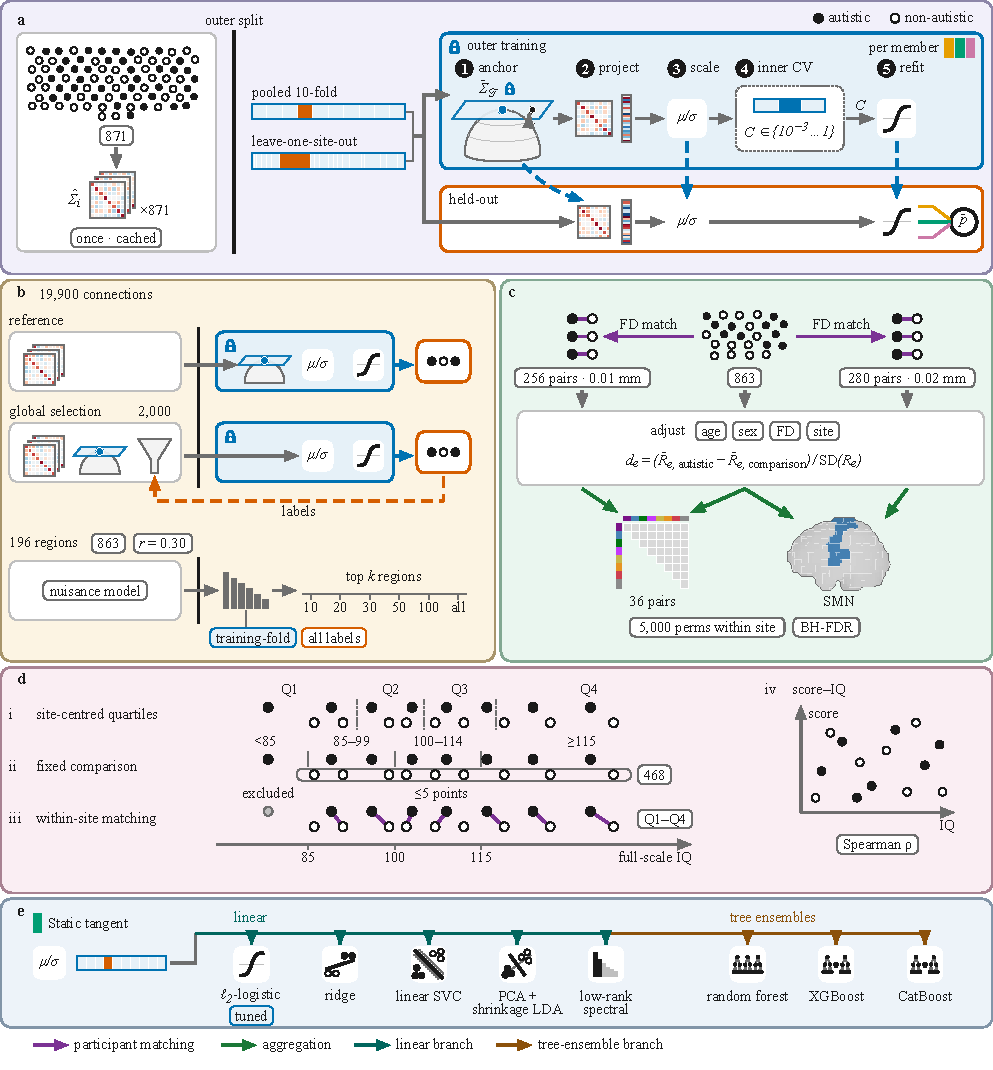
\includegraphics[width=\linewidth,height=0.78\textheight,keepaspectratio]{fig_designs}
\caption{Evaluation and analysis designs are summarised across five panels. (a) Nested CV is performed within each outer training partition through \ding{202}~anchor estimation (tangent reference), \ding{203}~projection, \ding{204}~scaling, \ding{205}~inner-CV tuning, and \ding{206}~refitting. (b) Feature selection is compared when performed within training folds and when all labels are used. (c) Group differences are evaluated after matching for head motion. (d) IQ-related analyses include (i)~quartiles, (ii)~a fixed comparison group, (iii)~matching, and (iv)~score--IQ correlation. (e) Classifier families include logistic regression, ridge, linear support-vector classification (SVC), shrinkage linear discriminant analysis (LDA) after principal component analysis (PCA), low-rank spectral classification, random forest, XGBoost, and CatBoost.}
\label{fig:designs}
\end{figure}

The classifier is then tuned and refitted on the transformed training data. To this end,
$C$ is selected by inner CV on the transformed training matrix. The selected
classifier is then refitted to the complete outer training partition, so that the final
model uses every training participant. Next, probabilities are predicted for the held-out
partition. Finally, the three member probabilities are combined. Per-participant covariance estimation is handled separately from these fold specific
steps. Each covariance estimate depends only on that participant's time series. Therefore,
it is cached before fold specific fitting without using information from other
participants. Shared quantities, in contrast, are estimated from several participants. For
this reason, shared references, scalers, feature selectors, and classifier parameters are
estimated at the training level specified for each analysis.

\subsubsection{Performance measures and aggregation}
\label{subsubsec:performance-measures}

Discrimination is assessed primarily using AUROC and the area under the precision--recall curve, both derived from continuous prediction scores. Threshold-based performance is also reported at 0.5 using accuracy, balanced accuracy, sensitivity, specificity, F1 score, and Matthews correlation coefficient, with autistic participants treated as the positive class. Balanced accuracy and Matthews correlation coefficient are included because they are less sensitive to unequal group sizes. Across the outer folds, performance is summarised in two ways: participant-pooled metrics are calculated from all concatenated out-of-fold predictions, while unweighted fold means and SDs give equal weight to each fold. Both summaries are retained because site sizes vary substantially in LOSO validation. In LOSO validation each fold is one site, so the fold mean gives equal weight to each site, whereas the participant-pooled value gives equal weight to each participant. Fold-level AUROC and accuracy are used in the planned comparison tables, whereas pooled out-of-fold predictions are used for calibration, paired prediction tests, and the main interval estimates.

\subsubsection{Interval construction}
\label{subsubsec:interval-construction}

Intervals are reported for the main performance measures. AUROC intervals are derived from the DeLong variance, while Wilson intervals are used for accuracy, sensitivity, and specificity. These intervals are based on the observed out-of-fold predictions and do not account for variation from repeating the full modelling procedure. Site-level variation is assessed using AUROCs from LOSO validation. Site-specific AUROCs are combined with a DerSimonian--Laird random-effects model, including only sites that contain both diagnostic groups. This leaves $J$ sites for analysis. Each site is weighted by $1/(V_j+\hat{\tau}^2)$, where $V_j$ is the DeLong variance and $\hat{\tau}^2$ is the estimated between-site variance. Because $V_j$ depends on the site's own AUROC, sites with higher AUROC receive more weight, and the random-effects mean is therefore compared descriptively with the unweighted and size-weighted means of the site AUROCs. Between-site heterogeneity is summarised using Cochran's $Q$ and $I^2$. The spread of the site estimates around the random-effects mean is then described by the 95\% interval in Equation~\eqref{eq:prediction-interval}:

\begin{equation}
\hat{\mu}
\pm
t_{0.975,\,J-2}
\sqrt{\hat{\tau}^2+\operatorname{SE}(\hat{\mu})^2}.
\label{eq:prediction-interval}
\end{equation}

Here, $\hat{\mu}$ is the random-effects mean AUROC and
$\operatorname{SE}(\hat{\mu})$ is its standard error. By incorporating both uncertainty in
the pooled mean and estimated between-site variation, the interval summarises descriptive variation among the ABIDE-I site estimates.

The site-specific estimates are not independent studies, because each is produced by a model
trained on the remaining 19 sites, so any two training sets overlap in almost all of their
participants. The random-effects model does not represent this dependence, and the
between-site variance is therefore understated. For this reason the random effects mean and
the interval are reported as descriptive summaries of variation among the ABIDE-I site
estimates. Neither quantity is interpreted as the performance expected at a new acquisition
site, and the site-clustered bootstrap of Section~\ref{subsubsec:paired-comparisons} is used
where an interval on overall performance is required.



\subsubsection{Secondary fully nested penalty selection}
\label{subsubsec:nested-penalty}

In the primary penalty search, the tangent reference and feature scaler are fitted once on each outer training partition and then reused across the inner folds. This means that inner-validation participants contribute to these fitted transformations, although their diagnostic labels are not used. A fully nested sensitivity analysis removes this dependence by refitting the tangent reference and scaler within each of the three inner training folds and applying them only to the corresponding inner validation fold. Penalty strength is selected using the same procedure as in the primary analysis: stratified three-fold splitting without shuffling, mean inner AUROC, and the smaller value in the event of a tie. Because the primary search selects the lower boundary of the original grid, 0.001, the fully nested search is extended down to $10^{-5}$ to determine whether a smaller value is preferred. When the selected penalty differs from the primary choice, the corresponding model is refitted on the full outer training partition and the ensemble predictions are recomputed. Sensitivity is then assessed by the number of changed penalty selections and by the resulting changes in participant-pooled AUROC and accuracy.

\subsection{Probability assessment}
\label{subsec:probability-assessment}
The reliability of the ensemble probabilities is examined through calibration and within-training-partition recalibration. These probability analyses are added after the primary discrimination results are examined, as specified in Section~\ref{subsubsec:analysis-status}. Confidence-based abstention is described in the Supplementary Material.

\subsubsection{Primary descriptive assessment of calibration}
\label{subsubsec:calibration-assessment}

Beyond discrimination, the ensemble probabilities are assessed for calibration. The native probabilities from Equation~\eqref{eq:probability-ensemble} are first evaluated without recalibration by comparing predicted probabilities with observed outcome frequencies. For the primary ECE analysis, predictions are divided into ten equal-width bins, and the mean predicted probability in each bin is compared with the observed proportion of autistic participants. The resulting bin-level differences are combined into the expected calibration error (ECE), weighted by bin size \citep{Naeinietal2015,Guoetal2017}, as defined in Equation~\eqref{eq:calibration-error}. Because ECE alone does not fully characterise calibration, the Brier score, calibration slope, and calibration-in-the-large are also reported. The Brier score summarises the mean squared difference between predicted probabilities and observed outcomes, while the calibration slope and calibration-in-the-large assess the spread and overall level of the predicted probabilities, respectively. These measures are reported with the site-clustered bootstrap intervals described in Section~\ref{subsubsec:paired-comparisons}. Sensitivity to the ECE binning choice is further examined using 5, 10, and 20 equal-width bins, with the smallest number of participants per bin reported for each setting.

\begin{equation}
\operatorname{ECE}
=
\sum_{b=1}^{10}
\frac{|\mathrm{B}_b|}{n}
\left|
\frac{1}{|\mathrm{B}_b|}
\sum_{i\in\mathrm{B}_b}p_i^{\mathrm{ens}}
-
\frac{1}{|\mathrm{B}_b|}
\sum_{i\in\mathrm{B}_b}y_i
\right|.
\label{eq:calibration-error}
\end{equation}

In Equation~\eqref{eq:calibration-error}, $\mathrm{B}_b$ denotes the set of participants in bin $b$,
$n$ denotes the total number of participants, and $y_i=1$ denotes an autistic participant.
In this sum, empty bins contribute no term. Because ECE is computed from the probability of
the autistic class, it assesses positive-class probability calibration. In addition, the
same bin-level quantities are displayed in reliability diagrams under both validation
protocols. In such a diagram, the mean predicted probability of each bin is plotted against
the observed proportion of autistic participants in that bin. These diagrams are included
because they show in which probability range any disagreement occurs, whereas a single ECE
value does not.

\subsubsection{Primary descriptive recalibration within training partitions}
\label{subsubsec:recalibration}

The native ensemble probabilities are first assessed and are then recalibrated within each outer training partition so that the held-out labels do not influence the correction. Each outer training partition is divided into five internal parts. These parts are stratified by diagnosis under pooled validation and consist of whole sites under LOSO validation. For each split, the complete ensemble, including the tangent reference, feature scaler, and selected penalty strength, is refitted on four parts and used to predict the fifth. This produces a cross-fitted probability for every participant in the outer training partition, and only these probabilities and their diagnostic labels are used to estimate the recalibration. Three corrections are compared. The primary correction applies a constant shift to the probability logit, as given by Equation~\eqref{eq:recalibration-intercept}:
\begin{equation}
\operatorname{logit}\!\left(p_i^{\mathrm{rec}}\right)
=
\operatorname{logit}\!\left(p_i^{\mathrm{ens}}\right) + a .
\label{eq:recalibration-intercept}
\end{equation}
In Equation~\eqref{eq:recalibration-intercept}, $p_i^{\mathrm{ens}}$ is the native ensemble probability from Equation~\eqref{eq:probability-ensemble}, and $a$ is the fitted intercept offset. This correction is designated as primary because it adjusts the overall probability level with a single parameter while preserving the within-fold ranking of participants. A second correction also allows the probability spread to change, as given by Equation~\eqref{eq:recalibration-logistic}:
\begin{equation}
\operatorname{logit}\!\left(p_i^{\mathrm{rec}}\right)
=
a + b\,\operatorname{logit}\!\left(p_i^{\mathrm{ens}}\right).
\label{eq:recalibration-logistic}
\end{equation}
Here, $a$ and $b$ are estimated by logistic regression on the cross-fitted training probabilities. A third correction uses isotonic regression to learn a non-decreasing mapping from predicted probabilities to observed outcome frequencies \citep{ZadroznyElkan2002}. Its outputs are restricted to 0.005--0.995 to keep the logarithmic loss finite. Logistic and isotonic recalibration are treated as sensitivity analyses. A separate diagnostic examines whether the probability offset is related to intercept penalisation in the \texttt{liblinear} solver \citep{Fanetal2008}. Each ensemble member is therefore refitted on the outer training partition with the same penalty strength but an unpenalised intercept using the L-BFGS solver \citep{Pedregosaetal2011}. These probabilities are evaluated in the same way but are not used as a recalibration method. Every probability version is assessed on the corresponding held-out fold using ECE from Equation~\eqref{eq:calibration-error}, the Brier score, calibration slope, calibration-in-the-large, Brier skill score, logarithmic loss, and AUROC \citep{VanCalsteretal2019,Steyerbergetal2010}. Accuracy, sensitivity, and specificity at a threshold of 0.5 are also reported because recalibration can change threshold-based decisions even when participant ranking is preserved. Site-clustered bootstrap intervals are obtained as described in Section~\ref{subsubsec:paired-comparisons}, and differences from the native probabilities are calculated within the same bootstrap resamples. The corrections are not refitted within these resamples, so the intervals describe uncertainty in their evaluation rather than in recalibration fitting. Finally, calibration-in-the-large is estimated separately for sites with at least 30 participants, with Wald intervals obtained from the offset model. Between-site variation is summarised by the SD and $I^2$ using the DerSimonian--Laird estimator described in Section~\ref{subsubsec:interval-construction}. These site-level summaries describe heterogeneity within the observed cohort rather than performance at a new site.

\subsection{Interpretation of the linear members}
\label{subsec:interpretation}

This subsection examines which functional-system pairs contribute to the predictions of the linear ensemble members and how reproducible these patterns are. Because each member is linear, its score can be decomposed exactly across individual connections and then aggregated into the 36 pairs formed by the eight functional systems defined in Section~\ref{subsec:group-differences}. System-pair attribution is used to provide a more stable summary than individual connections. The analyses quantify pair-level contributions, assess the reproducibility of fitted patterns, compare them with permutation references and other analyses, and examine whether the highest-ranked pairs influence prediction on held-out participants. The evidential status of each analysis is stated in its heading.

\subsubsection{Secondary attribution of the score to system pairs}
\label{subsubsec:pair-contributions}

For participant $i$, the score from each linear ensemble member is decomposed across system pairs using Equation~\eqref{eq:score-decomposition}:
\begin{equation}
s_i
=
b + \sum_{j} w_j z_{ij}
=
b + \sum_{g} c_{ig},
\qquad
c_{ig} = \sum_{j\in g} w_j z_{ij}.
\label{eq:score-decomposition}
\end{equation}
Here, $b$ is the intercept, $w_j$ is the weight of standardised connection $j$, $z_{ij}$ is its value for participant $i$, and $c_{ig}$ is the contribution of system pair $g$. The summed pair contributions are checked against the stored model score for each participant. For a linear model, the Shapley value of a feature is $w_j\left(z_{ij}-\mathbb{E}[z_j]\right)$ \citep{LundbergLee2017}, so pair-level Shapley sums differ from $c_{ig}$ only by a participant-independent constant that cancels in group comparisons. Pair contributions are therefore calculated directly for each held-out participant using the features and model weights fitted without that participant. They are summarised by the mean contribution difference $d_g$ between autistic and non-autistic participants, its share of the total score separation, and its value per connection. A site-adjusted version is also obtained by estimating the group difference within each site and combining sites using weights based on the two group sizes. In addition, the AUROC of $c_{ig}$ alone is calculated to measure the discrimination provided by each pair. These summaries are evaluated separately for the three connectivity views and are also averaged across views with equal weight as an approximation to the probability-based ensemble. This approximation is checked by comparing the averaged member scores with the probability-mean ensemble through their Spearman correlation, their participant-pooled AUROCs, the proportion of participants classified differently at the 0.5 threshold, and the separation between the groups on the logit scale. Connections involving the four excluded regions are retained in a separate unassigned category, and intervals are obtained using the site-clustered bootstrap described in Section~\ref{subsubsec:paired-comparisons}.

\subsubsection{Secondary reproducibility of the fitted patterns}
\label{subsubsec:pattern-reproducibility}

Because linear-model weights reflect the joint use of correlated features, they are not interpreted directly as group differences \citep{Haufeetal2014}. The fitted pattern is therefore also represented by the structure coefficient in Equation~\eqref{eq:structure-coefficient}:
\begin{equation}
r_j = \operatorname{corr}\!\left(z_{\cdot j},\, s_{\cdot}\right).
\label{eq:structure-coefficient}
\end{equation}
Here, $r_j$ is the Pearson correlation between standardised connection $j$ and the model score across participants in a training sample, and is proportional to the activation pattern described by \citet{Haufeetal2014}. Weights and structure coefficients are examined at the connection, region, and system-pair levels, with regional and pair-level values obtained by averaging the corresponding signed connection values. Reproducibility is assessed first by comparing all pairs of outer training partitions with Spearman correlation, giving 45 comparisons under pooled validation and 190 under LOSO validation. Because these partitions overlap, this analysis reflects fitting stability rather than independent replication. Independent reproducibility is then assessed over 40 random split-half divisions stratified by site and diagnosis, so that every site contributes to both halves. Each half is fitted independently from tangent-reference estimation through classification, with the penalty fixed at 0.001, the value selected in every outer fold of the primary analysis. Agreement between halves is measured using Spearman correlation for both weights and structure coefficients at all three levels, together with the proportion of features having the same structure-coefficient sign. Each connectivity view is analysed separately.

\subsubsection{Secondary permutation reference}
\label{subsubsec:interpretation-permutation}

Permutation analysis is used to provide reference distributions for pattern reproducibility and system-pair AUROC. Diagnostic labels are permuted within site so that site-specific diagnostic proportions are preserved. For outer-fold reproducibility, pooled ten-fold validation is repeated over 100 permutations with the penalty fixed at the value selected from the observed labels. For the independent split-half analysis, 30 within-site permutations are performed for each split, and the results are averaged across splits to obtain one reference value per permutation. Observed reproducibility is compared with the 95th percentile of this reference distribution, and the corresponding $p$-value is the proportion of reference values, including the observed value, that are at least as large. The minimum attainable $p$-value for the split-half analysis is therefore $1/31$. For system-pair AUROC, familywise correction is applied by recording the maximum absolute deviation from 0.5 across all 36 pairs in each permutation. A pair-specific $p$-value is then calculated as the proportion of permutations for which this maximum is at least as large as the observed deviation for that pair. This procedure treats the 36 system-pair tests as one family.

\subsubsection{Secondary reproducibility across sites}
\label{subsubsec:site-disjoint}

\addhl{Reproducibility across sites is assessed over 40 random divisions of the 20 sites into two halves of 10 sites, so that no site contributes to both halves. A division is admitted when each half holds 42 to 58\% of the participants and the autistic proportions of the halves differ by at most 0.08. Each half is analysed as in the split-half procedure above, in two variants: with the classifier of the primary analysis, and after regressing the site indicators of the half, age, sex, and mean FD out of every standardised feature. The reference is the 95th percentile, over 30 within-site permutations of diagnosis, of the agreement averaged across the 40 divisions. The criterion was fixed before the analysis: the system-pair structure-coefficient agreement between halves must exceed the 95th percentile of the permutation reference in at least two of the three views, for each variant.}

\subsubsection{Exploratory agreement across views and with the group-difference analysis}
\label{subsubsec:interpretation-agreement}

Agreement is examined across the three connectivity views and between the classifier patterns and the nuisance-adjusted group-difference results. Across views, Spearman correlations are calculated between the mean structure coefficients of the 36 system pairs and, separately, between those of the retained regions. Agreement with the group-difference analysis is assessed by correlating each pair's mean structure coefficient with its corresponding standardised group difference from both the full-cohort and motion-matched analyses defined in Equation~\eqref{eq:group-difference}. The same comparison is performed for the 21 somatomotor regions using regional structure coefficients averaged over within-system connections. Because the group-difference analysis adjusts for site, motion, age, and sex, whereas the classifier does not, these correlations are interpreted as descriptive agreement between analyses. They are treated as exploratory because the system pairs and regions are not statistically independent.

\subsubsection{Exploratory deletion and retention of the highest-ranked pairs}
\label{subsubsec:deletion-retention}

The importance ranking of system pairs is evaluated by testing whether the highest-ranked pairs affect prediction on held-out participants. Within each training partition, the importance of pair $g$ is defined as its share of the training-score variance using Equation~\eqref{eq:importance}:
\begin{equation}
I_g
=
\frac{\sum_{j\in g} w_j\,\operatorname{cov}\!\left(z_{\cdot j},\, s_{\cdot}\right)}{\operatorname{var}\!\left(s_{\cdot}\right)}.
\label{eq:importance}
\end{equation}
The covariance and variance are calculated across the training participants, and the contributions of all connections sum to one. Held-out scores are then recomputed from Equation~\eqref{eq:score-decomposition} without refitting the model. Two analyses are performed: the $m$ highest-ranked pairs are either removed or retained alone, with $m$ set to 0, 1, 2, 3, 4, 6, 8, 12, 18, 24, 30, 35 and 36. AUROC is pooled across folds using the same procedure as in the primary analysis. Each result is compared with 200 reference draws in which the pair ranking is randomly permuted within each fold. This analysis tests whether the fitted model relies more strongly on its highest-ranked system pairs than expected from a random ranking. Connections in the unassigned category are retained in all conditions.

\subsection{Conditions for trustworthy use}
\label{subsec:trust-conditions}

\addhl{This subsection examines the conditions under which the recalibrated probabilities can be used, with the stored out-of-fold predictions of the primary ensemble and no refitting. These analyses were added after the primary results, and their status is stated in each heading (Section~}\ref{subsubsec:analysis-status}).

\subsubsection{Secondary site base rate and calibration at a new site}
\label{subsubsec:base-rate}

\addhl{Differences in calibration-in-the-large between withheld sites are examined as a possible consequence of differences in their autistic proportion. For a withheld site with autistic proportion $\pi_s$ and a training partition with proportion $\pi_{\mathrm{tr}}$, the recalibrated logit $z_i$ of each participant is shifted by Equation~}\eqref{eq:base-rate-shift} \citep{Saerensetal2002}:
\begin{equation}
z_i'
=
z_i
+
\log\frac{\pi_s}{1-\pi_s}
-
\log\frac{\pi_{\mathrm{tr}}}{1-\pi_{\mathrm{tr}}}.
\label{eq:base-rate-shift}
\end{equation}
\addhl{Only the intercept changes, so the ranking of participants is preserved. Because $\pi_s$ is computed from the labels of the withheld site, this shift identifies a mechanism and is not a deployable procedure. How accurately the proportion must be known is examined by changing it by errors from $-0.20$ to $+0.20$. Two procedures that do not use the true proportion are also examined: estimation of $\pi_s$ from the unlabelled predictions by expectation--maximisation} \citep{Saerensetal2002}\addhl{, and estimation of the proportion or of the intercept from $k=10$ or 15 labelled participants of the site, with shrinkage towards the training value, evaluated on the remaining participants over 500 random draws. For each scenario, heterogeneity across the 10 sites with at least 30 participants is summarised by $I^2$ and $\tau$ (Section~}\ref{subsubsec:interval-construction}\addhl{), together with the mean absolute site offset and the number of sites whose 95\% interval excludes zero.}

\subsubsection{Secondary operating points and net benefit}
\label{subsubsec:operating-points}

\addhl{Within each outer training partition, a threshold is chosen on the recalibrated inner cross-fitted predictions of the training participants only: the lowest threshold with a specificity of at least 0.80, the highest threshold with a sensitivity of at least 0.80, or the threshold that maximises the Youden index. The threshold is applied to the held-out fold, and sensitivity and specificity are calculated from the pooled held-out predictions with 95\% site-clustered bootstrap intervals. Because ABIDE-I has a higher autistic proportion (46\%) than a screening population, predictive values are also calculated at proportions of 3, 10, 25, and 46\% by Bayes' rule. Net benefit at threshold probability $t$ is $\mathrm{TP}/n-(\mathrm{FP}/n)\,t/(1-t)$} \citep{VickersElkin2006,VanCalsteretal2018}\addhl{, and the gain over treating all participants is compared for the recalibrated and the native probabilities at $t=0.30$, 0.40, and 0.50.}

\subsubsection{Exploratory stratified validation}
\label{subsubsec:strata}

\addhl{AUROC and calibration-in-the-large are calculated within strata of age (below 12, 12 to 17, and 18 years or above), mean FD (thirds of the cohort), and site size (fewer than 40, 40 to 79, and 80 or more participants), with site-clustered bootstrap intervals for AUROC and for its difference between the extreme strata. Calibration-in-the-large is also calculated after the shift of Equation~}\eqref{eq:base-rate-shift} \addhl{with the proportion of each stratum. Sex and IQ strata are reported with the cognitive analyses, and clinically referred comparison groups are not available in ABIDE-I.}

\subsection{Planned comparisons}
\label{subsec:planned-comparisons}
This subsection presents the planned primary, secondary, and exploratory comparisons built on the same prediction and validation framework. These analyses examine how performance and interpretation vary with connectivity representation, classifier choice, atlas and feature-selection strategy, phenotypic and site effects, participant subgroups, data availability, and model interpretability. Three secondary analyses (confidence-based abstention, combinations of brain parcellations, and label-noise sensitivity) are described in the Supplementary Material. 

\subsubsection{Primary descriptive comparison}
\label{subsubsec:primary-comparisons}

\paragraph{\textbf{Static and windowed connectivity.}}
\label{par:static-windowed}
The planned comparisons use the three-member prediction model under both pooled ten-fold and LOSO validation, with each analysis classified by its status in Section~\ref{subsubsec:analysis-status}. The first primary descriptive comparison evaluates static tangent connectivity against the dynamic mean while controlling the level of additional shrinkage. Because the windowed representation uses $r=0.15$, static tangent connectivity is evaluated at both $r=0$ and $r=0.15$, and the dynamic mean is compared directly with the $r=0.15$ static representation. Other representation-specific steps, including window sampling, covariance aggregation, and reference construction, remain unchanged. Static tangent performance is also examined across the shrinkage grid ${0,0.05,0.10,0.15,0.20,0.30,0.40,0.50,0.65,0.80}$. The sweep is first evaluated up to 0.30 and is later extended to 0.80 to examine stronger shrinkage, without changing the fixed $r=0.15$ comparison. In a separate nested analysis, the shrinkage level is selected within each outer training partition. The fixed and data-selected analyses are therefore reported separately, since one uses a predefined shrinkage level while the other estimates it from the training data. The difference between the windowed and the shrinkage-matched static model is also given with a site-clustered bootstrap interval (Section~\ref{subsubsec:paired-comparisons}).

\paragraph{\textbf{Feature-selection scope.}}
\label{par:selection-scope}
This primary descriptive comparison examines how model performance changes when fitted steps are allowed to access data beyond the outer training fold. Seven data-access conditions are evaluated using the 19,900 static tangent features from the primary cohort, while the same participants and outer folds are retained throughout. The reference condition fits the tangent reference, scaler, and classifier within each outer training fold. The global-reference condition estimates the tangent reference from all participants but retains fold-specific scaling, while the global-scaling condition fits both the reference and scaler globally. In the global-selection condition, the tangent reference is fitted globally, scaling remains fold-specific, and the 2,000 strongest connections are selected with an F test using all diagnostic labels. These features represent approximately 10\% of all connections. A held-out-tuning condition selects $C$ using the held-out fold, whereas a site-feature condition adds one-hot site indicators to the otherwise fold-specific pipeline. Finally, the combined condition applies global tangent projection, global scaling, global label-informed feature selection, held-out $C$ selection, and site indicators together. Here, ``global'' denotes any step fitted using all participants, including those in the held-out fold. The main connection-level conditions are illustrated in Figure~\ref{fig:designs}b.

The same question is also examined at the region level. This analysis uses the group-contrast cohort of 863 participants and 196 regions, with additional shrinkage fixed at $r=0.30$. The nuisance model is first fitted to the complete analysis cohort, after which each region is ranked by the average absolute group difference across its incident connections. Region ranking is performed either with all diagnostic labels or with labels restricted to the outer training fold, allowing the effect of label access to be isolated. Models are then fitted using the top 10, 20, 30, 50, or 100 ranked regions, while a model containing all retained regions serves as the reference condition.

In the published training-fold condition the regions are ranked inside each fold, but the nuisance adjustment used for that ranking is fitted once on the complete analysis cohort, so the held-out participants contribute to the residuals from which the ranking is derived. The condition is therefore repeated with the nuisance coefficients estimated from the outer-training rows alone and applied to those rows only, so that every data-dependent step of the selection sees training participants and nothing else. The folds, the connectivity features, the tangent projection, the feature scaling and the classifier are unchanged, so any difference is attributable to the nuisance fit.

\paragraph{\textbf{Pooled and within-participant symptom associations.}}
\label{par:symptom-associations}
This primary descriptive comparison examines whether out-of-fold ensemble probabilities are associated with six symptom measures. These include the ADOS total and calibrated severity scores, the ADI-R social, verbal-communication, and restricted/repetitive-behaviour domain scores, and the Social Responsiveness Scale (SRS) total \citep{Lordetal1994}. Each analysis uses only participants with an available score for the corresponding instrument, and missing symptom values are not imputed.

Associations are measured using Spearman correlation and are evaluated at two levels. The pooled analysis includes all participants with an available symptom score, whereas the within-participant analysis is restricted to autistic participants. This second analysis is included because an association observed across both diagnostic groups partly reflects the difference between the groups rather than variation within autistic participants. Both analyses are performed using out-of-fold predictions from pooled ten-fold and LOSO validation.



\subsubsection{Secondary comparison}
\label{subsubsec:secondary-comparisons}

\paragraph{\textbf{Dynamic trajectory blocks.}}
\label{par:trajectory-blocks}
In this secondary comparison, the dynamic mean is evaluated both alone and together with dispersion and velocity. Two combination strategies are examined. In feature concatenation, the mean is combined with dispersion, with velocity, or with both, and a single classifier is fitted to each joined feature vector. In late fusion, separate classifiers are fitted to the individual trajectory blocks and their predicted probabilities are averaged with equal weights. These approaches are compared because concatenation applies one regularisation penalty across all included features, whereas late fusion allows each block to be modelled separately. Standalone performance is reported for the dynamic mean, while dispersion and velocity are evaluated only as part of the combined conditions.

\paragraph{\textbf{Classifier configurations.}}
\label{par:classifier-family}
Eight classifier configurations are compared using the same static tangent features, feature scaling, and outer validation folds. This common setup ensures that performance differences are not caused by changes in the input features or participant partitions. Five linear or low-rank models are evaluated: nested $\ell_2$-regularised logistic regression; ridge classification with penalty strength 100; linear SVC with $C=0.01$; shrinkage LDA after PCA reduction to 200 components; and a rank-20 two-stage low-rank spectral classifier, which is specified below. Three tree ensembles are also included. Random forest uses 300 trees with unrestricted depth, XGBoost uses 300 trees with maximum depth 4, learning rate 0.1, row subsampling 0.8, and column subsampling 0.3, and CatBoost \citep{Prokhorenkovaetal2018} uses 300 trees with depth 4, learning rate 0.1, and feature subsampling 0.3. The linear and tree-based configurations are summarised in Figure~\ref{fig:designs}e. Hyperparameter tuning is applied only to the logistic model because it is the classifier used in the primary ensemble. Its $C$ value is selected from $\{0.001,0.01,0.1,1.0\}$ using three-fold stratified CV within each outer training partition. All other classifiers are evaluated with fixed configurations. The analysis is therefore treated as a secondary comparison of the specified configurations rather than a comparison of the best attainable performance of each classifier family. Before threshold-based metrics are calculated, all model outputs are placed on a common zero-to-one scale. For classifiers without \texttt{predict\_proba}, the decision score is transformed with a logistic function, allowing the same decision threshold to be applied across classifiers.

\paragraph{\textbf{Phenotype model.}}
\label{par:phenotype-model}
In this secondary comparison, a phenotype-only model is fitted using age, sex, full-scale IQ, verbal IQ, performance IQ, and handedness. Missing values are imputed using medians estimated from the outer training partition, after which the variables are standardised and entered into logistic regression. The resulting phenotype probability is evaluated both on its own and as an additional member of the imaging ensemble. This allows the contribution of phenotype information to be examined separately from the discrimination provided by the imaging models.

\paragraph{\textbf{ComBat harmonisation.}}
\label{par:combat-harmonisation}

In this secondary comparison, ComBat harmonisation is used to reduce site-related shifts in feature means and variances \citep{Johnsonetal2007,Fortinetal2018}. Site is treated as the batch variable, while age and sex are retained as covariates and diagnosis is excluded so that harmonisation does not depend on the prediction target. ComBat is fitted separately within each outer fold after feature scaling. The training features and the complete unlabelled held-out batch are supplied jointly so that a batch effect is estimated for a site that is absent from the training data. This is a transductive batch-level analysis because it requires simultaneous access to the full unlabelled held-out site; it is not an inductive test for a single participant arriving from an unseen site. If age or sex were missing, age would be replaced by the training median and sex would be assigned to the male category, although these rules are not required in the primary cohort. When ComBat-transformed features are unavailable, the scaled features are retained under a prespecified fallback so that every outer fold still contributes predictions.


\paragraph{\textbf{Low-rank spectral approximation.}}
\label{par:low-rank-spectral}
In this secondary analysis, a linear classifier is approximated with a small number of
spectral components of its weight matrix, that is, with a low-rank spectral approximation.
To this end, each standardised static tangent feature vector is represented as the upper
triangle of a symmetric matrix $\widetilde{S}_i$. In the same way, a dense linear
coefficient vector, that is, one with a non-zero weight for every feature, is mapped to a
symmetric weight matrix $W$. The off-diagonal entries of $W$ are divided by two, so that
the matrix inner product matches the original vector dot product.

The weight matrix is then decomposed into its eigenvectors and eigenvalues, as given in
Equation~\eqref{eq:weight-eigendecomposition}:
\begin{equation}
W
=
U\Lambda U^\top.
\label{eq:weight-eigendecomposition}
\end{equation}

In Equation~\eqref{eq:weight-eigendecomposition}, the columns of $U$ are the eigenvectors of $W$, and the diagonal
matrix $\Lambda$ holds the eigenvalues. Each eigenvector, together with its eigenvalue,
forms one component. The components are ordered by the absolute value of their eigenvalues.
This ordering places first the components that contribute most to the weight matrix. For
rank $q$, that is, when $q$ components are retained, the first $q$ components then define
the participant scores in Equation~\eqref{eq:component-scores}:
\begin{equation}
z_{ik}
=
u_k^\top \widetilde{S}_i u_k,
\qquad k=1,\ldots,q.
\label{eq:component-scores}
\end{equation}

In Equation~\eqref{eq:component-scores}, $u_k$ is the $k$th column of $U$, and $z_{ik}$ is the score of
participant $i$ on component $k$. The scores in Equation~\eqref{eq:component-scores} are obtained from a
dense stage-one logistic model with $C=0.01$. Next, a second logistic regression with
$C=1.0$ is fitted to the component scores. This two-stage design is used so that the final
classifier operates on the $q$ component scores alone. The ranks $\{1,2,5,10,20,30,50,100\}$
are evaluated on the same folds, so that differences between ranks do not reflect different
data partitions. In a separate spectral analysis, the cumulative squared-singular-value mass
of the feature matrix and the cumulative absolute eigenvalue mass of $W$ are recorded. Both
masses describe how quickly the total is accumulated as components are added.

\subsubsection{Exploratory comparison}
\label{subsubsec:exploratory-comparisons}

\paragraph{\textbf{Cognitive and sex subgroups.}}
\label{par:cognitive-sex-subgroups}
Discrimination across cognitive ability and sex is examined using out-of-fold predictions from the primary cohort. Predictions are first linked to the verified participant and site records. Cognitive effects are evaluated in three complementary ways. First, full-scale IQ is centred within site and divided into quartiles, and AUROC is calculated within each quartile. Second, autistic participants are divided into full-scale IQ bands below 85, 85--99, 100--114, and 115 or above, while the same 468 non-autistic participants form the comparison group for every band. Third, autistic and non-autistic participants are matched within site on full-scale IQ using greedy nearest-neighbour matching without replacement and a maximum difference of five IQ points. Unmatched autistic participants are excluded, and AUROC is then estimated within site-centred IQ quartiles of the matched sample. These designs are summarised in Figure~\ref{fig:designs}d. Additional analyses examine full-scale, verbal, and performance IQ separately within autistic and non-autistic participants. Site, age, and mean FD are regressed from both classifier score and IQ before Spearman correlation is calculated. Sex-specific AUROCs are reported only for subgroups containing at least 20 participants and both diagnostic classes.

\paragraph{\textbf{Cohort definition.}}
\label{par:cohort-definition}
Sensitivity to cohort definition is examined by evaluating the same model specifications in two samples. The static tangent classifier and primary three-member ensemble are first tested in the 871-participant primary cohort and then in the wider QC cohort of 1,032 participants. No modelling choices are changed between cohorts, so observed differences reflect cohort composition rather than a different analysis pipeline. The static tangent classifier is evaluated with pooled ten-fold validation, while the primary ensemble is evaluated with both pooled ten-fold and LOSO validation.

\paragraph{\textbf{Scan duration and sample size.}}
\label{par:duration-sample-size}
The effect of scan duration is examined among participants with at least 232 volumes. The same scans are truncated to 40, 60, 90, 120, 160, 200, and 232 volumes so that the participant sample remains fixed across durations. Covariance matrices are re-estimated at each duration, and additional shrinkage values of 0.15, 0.30, and 0.50 are tested to account for less stable covariance estimation in shorter scans. A separate sample-size analysis uses full-length scans with subsets of 100, 200, 300, 400, 550, 700, and 825 participants. One unstratified random subset is drawn at each size, with additional shrinkage fixed at $r=0.15$ so that only sample size varies. Sample size is also examined within the New York University (NYU) site using five-fold validation to reduce between-site variation. The association of scan duration and sample size with AUROC is summarised using Spearman correlation (Section~\ref{subsubsec:correlation-analyses}).

\paragraph{\textbf{Training-cohort homogeneity.}}
\label{par:training-homogeneity}
The effect of training-cohort homogeneity is examined by comparing models trained on one site with models trained across several sites. NYU is used as the single-site source, and a static tangent model with additional shrinkage $r=0.30$ is fitted. Four conditions combine one-site or multi-site training with same-site or other-site testing. In each condition, 120 training participants and 40 test participants are sampled without class stratification across 20 random repetitions. Sample sizes are kept equal across conditions, so the main difference is the site composition of the training and test sets. AUROC is used as the outcome in all four conditions.

\paragraph{\textbf{Component--symptom associations.}}
\label{par:component-symptom}
A rank-20 spectral classifier is fitted once to the complete primary cohort so that all participants are represented in a common component space. The tangent reference, scaler, and classifier are estimated from the full cohort and its diagnostic labels, while symptom measures are used only in the subsequent association analysis. Within autistic participants, age, sex, full-scale IQ, and site are regressed from both the component scores and symptom measures. Spearman correlation is then calculated between the resulting residuals, with p-values adjusted across all component--instrument combinations. Because these associations depend on components from a single full-cohort fit, component stability is assessed separately. Components estimated within each CV training fold are matched to those from the full cohort, and stability is summarised by the highest absolute cosine similarity for each component. The absolute value is used because eigenvector sign is arbitrary.

\subsection{Exploratory group-difference analyses}
\label{subsec:group-differences}

\subsubsection{Connection construction and nuisance adjustment}
\label{subsubsec:connection-adjustment}

The group-difference analyses are used to compare functional connectivity between autistic and non-autistic participants. These exploratory analyses are conducted in the group-contrast cohort of 863 participants using 196 retained regions. Pairwise Pearson correlations are Fisher transformed and vectorised before analysis. For each connection, a linear nuisance model is fitted using age, sex, mean FD, and acquisition-site indicators. The adjusted connectivity values are then used for group comparison. Missing nuisance values are replaced with the cohort median so that all participants are retained.


Standardised group differences are then calculated from the residual connection values.
For connection $e$, the effect is defined by Equation~\eqref{eq:group-difference}:
\begin{equation}
d_e
=
\frac{
\overline{R}_{e,\mathrm{autistic}}
-
\overline{R}_{e,\mathrm{comparison}}
}{
\operatorname{SD}(R_e)
}.
\label{eq:group-difference}
\end{equation}

In Equation~\eqref{eq:group-difference}, $\operatorname{SD}$ is calculated from the residuals across both groups, and the barred terms denote the corresponding group means. Non-autistic participants are used as the comparison group, so negative values indicate lower connectivity in autistic participants. By standardising with the pooled residual variation, connection effects are placed on a common scale and can be compared and averaged.


\subsubsection{Exploratory system, motion-matched, and regional analyses}
\label{subsubsec:system-motion-regional}

Connection-level group effects are first summarised at the functional-system level by grouping connections according to the systems of their two endpoints. For each system pair containing at least 20 connections, the standardised connection effects are averaged to obtain a system-level effect. Because diagnosis is associated with age, sex, and mean FD, inference uses Freedman--Lane residual permutation with 5,000 within-site permutations under seed 42 and BH-FDR correction across system pairs. In this procedure, a reduced nuisance model is fitted first, its residuals are permuted within site and added back to the fitted values, and the full model is then refitted while the diagnosis vector remains fixed. This provides a covariate-adjusted permutation reference for both system-level and regional effects, and the Freedman--Lane effect is the resulting diagnosis coefficient in units of the residual SD. As a sensitivity analysis, the standardised differences of the residualised connections are also tested by permuting diagnostic labels within site (5,000 permutations, seed 42, BH-FDR across system pairs). Sensitivity to head motion is examined separately by matching autistic and non-autistic participants within site on mean FD using greedy matching without replacement. Missing nuisance values are imputed from the complete pre-matching cohort. A 0.01 mm caliper is used for the system analysis, retaining 256 matched pairs, while a 0.02 mm caliper is used for the regional analysis, retaining 280 pairs. Nuisance adjustment and permutation testing are repeated within each matched cohort, and the remaining motion difference is assessed with the Mann--Whitney U test before and after matching (Figure~\ref{fig:designs}c). The relation between motion and overall connectivity is examined independently by correlating mean FD with the participant-wise mean Fisher-transformed connectivity across the 19,110 retained connections. Spearman correlation is calculated both before and after regressing acquisition site from the two variables. The relation is also examined within the somatomotor system by correlating mean FD, after removing site from both variables, with each of the 210 within-somatomotor connections, and by multiplying the site-adjusted regression slope of each connection on mean FD by the difference in mean FD between autistic and non-autistic participants, which gives the group difference that this linear relation would produce. Regional analysis is then performed within the selected functional system, with the somatomotor system used as the default. Each parcel is assigned the mean standardised group difference across its within-system connections, and BH-FDR correction is applied across the tested regions. Because the system is selected after inspection of the system-level results, and the correction across its regions does not account for that selection, the regional analysis remains exploratory and descriptive. Internal stability is assessed with 200 independent split-half repetitions in which nuisance adjustment and regional effects are refitted separately in each half and the resulting rankings are compared using Spearman correlation. The same procedure is applied to all within-system connections and to the top 50 connections. As a reference, 100 random region sets of the same size are evaluated using the first 50 split-half repetitions to determine whether the observed regional ranking is more stable than similarly sized sets elsewhere in the brain.

\subsection{Statistical analysis}
\label{subsec:statistical-analysis}

\subsubsection{Analysis status and multiplicity}
\label{subsubsec:analysis-status}

All prediction and group-difference analyses are interpreted within a common evidential framework, with no predefined confirmatory hypothesis-testing family. Analyses are instead classified as primary descriptive, secondary, or exploratory, and their status is stated in the relevant headings. Primary descriptive analyses include the primary-cohort ensemble, the shrinkage-matched comparison of static and windowed connectivity, feature-selection scope, pooled and within-autistic-group symptom associations, and assessment and recalibration of the ensemble probabilities. Pairwise model comparisons are therefore interpreted descriptively rather than as confirmatory tests. Inference for the group-difference analyses uses Freedman--Lane residual permutation, with the within-site permutation of residualised connections as a sensitivity analysis, and the regional analysis within the selected system is descriptive because the system is chosen from the same data. \addhl{The analyses of base rate and operating points and the reproducibility across sites are secondary, the stratified validation is exploratory, and the criterion for reproducibility across sites was fixed before that analysis was run.} System-pair attribution, pattern reproducibility, and fully nested penalty selection are treated as secondary analyses, whereas agreement with group-difference results and the deletion and retention analyses are exploratory. The calibration and interpretation analyses were added after examination of the primary discrimination results in response to review, and this sequence is reported to make their evidential status explicit. Multiplicity is handled according to analysis type. Pairwise comparison p-values are reported without adjustment together with effect sizes, while BH-FDR q-values are provided only for reference. BH-FDR correction is applied to related families of network, regional, symptom-association, and component--symptom tests. For symptom analyses, the six measures form one testing family within each combination of validation protocol and correlation scope. For system-pair AUROCs, familywise $p$-values are obtained from the maximum statistic across all 36 pairs under permutation (Section~\ref{subsubsec:interpretation-permutation}), so no additional BH-FDR correction is applied.

\subsubsection{Paired predictive comparisons}
\label{subsubsec:paired-comparisons}

Predictive conditions evaluated on the same participants are compared using their stored out-of-fold predictions. AUROC differences are tested with DeLong's test, while differences in binary classifications at the 0.5 threshold are assessed with McNemar's test. Site-clustered bootstrap intervals are also reported because DeLong and Wilson intervals based on pooled out-of-fold predictions treat participants within the same acquisition site as independent and condition on a single fitted split structure. For the bootstrap, the 20 site labels are resampled with replacement 2,000 times using random seed 42, with all participants from each sampled site retained together. The performance measure is recomputed in each resample, and percentile intervals are obtained from the resulting distribution. These intervals therefore account for site-level clustering and are reported alongside the DeLong and Wilson intervals. The parametric intervals are interpreted as narrower estimates of uncertainty rather than as complete accounts of site-level dependence.

\subsubsection{Permutation analyses}
\label{subsubsec:permutation-analyses}

Functional-system and regional analyses use 5,000 within-site permutations. In the Freedman--Lane analysis the residuals of the reduced nuisance model are permuted, and in the sensitivity analysis the diagnostic labels are permuted. Permuting within each site preserves the number of autistic and non-autistic participants at that site while generating the null distribution for the group effect. Two-sided p-values use the plus-one adjustment in Equation~\eqref{eq:permutation-p}, where $T_{\mathrm{obs}}$ is the observed system- or region-level effect and $T_b^\ast$ is the corresponding effect under permutation $b$:
\begin{equation}
p
=
\frac{
1
+
\sum_{b=1}^{B}
\mathbb{1}\left(
\left|T_b^\ast\right|
\geq
\left|T_{\mathrm{obs}}\right|
\right)
}{
B+1
},
\qquad B=5000.
\label{eq:permutation-p}
\end{equation}
Here, $B$ is the number of permutations and $\mathbb{1}(\cdot)$ equals one when its condition is satisfied and zero otherwise. The plus-one adjustment includes the observed labelling among the possible outcomes, giving a minimum attainable value of $1/5001$ when $B=5000$; values at this limit are reported as $p < 2\times10^{-4}$.

\subsubsection{Correlation analyses}
\label{subsubsec:correlation-analyses}

Spearman rank correlation is used for symptom, cognitive-subgroup, motion--connectivity, internal-stability, and scaling analyses. It is used because these analyses concern monotonic associations and do not require a linear relation or normally distributed variables. Each reported correlation is accompanied by its participant scope, available sample size, and any adjustment procedure, because these differ across analyses and affect interpretation.


\subsection{Reproducibility and scope}
\label{subsec:reproducibility-scope}

Reproducibility is supported by fixed random seeds, stored fold-level outputs, and retained out-of-fold predictions. Participant labels and site codes are verified whenever predictions are linked to phenotypic variables or used in paired analyses. The scope of each finding is defined by the corresponding cohort and analysis setting. Primary discrimination is evaluated in the 871-participant ABIDE-I cohort, cohort-sensitivity analyses use the wider QC cohort of 1,032 participants, and group-difference analyses use 863 participants and 196 retained regions. Generalisation is assessed only across the ABIDE-I acquisition sites and should therefore be interpreted within this multisite research setting. Dynamic analyses are limited to six windows of 50 volumes, whose durations vary across sites because repetition time is not harmonised. Group-level findings are also conditional on the C-PAC \texttt{filt\_noglobal} preprocessing pipeline, CC200 parcellation, nuisance adjustment, and recorded mean FD. The computational environment is recorded with the results: Python 3.12.8, NumPy 2.4.6, pandas 3.0.3, SciPy 1.18.0, and scikit-learn 1.8.0 on macOS (arm64), with random seed 42. The primary cohort identifiers are stored with the results and summarised by the SHA-256 digest \texttt{6c943ff4\ldots9b81a057} of their sorted list. Pooled folds are generated by stratified ten-fold splitting with shuffling under seed 42, while LOSO follows site labels in alphabetical order. Analyses added during review use the same seed, with diagnosis-stratified inner folds for pooled validation and site-grouped inner folds for LOSO validation. The permutation analysis uses 100 within-site permutations with seeds derived from 42, and the independent split-half analysis uses 40 random divisions with 30 permutations each. A sequential analysis driver validates each stage before the next begins, and refitting reproduces the stored out-of-fold predictions to within $2.1\times10^{-7}$. Code and result files are prepared for public release under the ABIDE data-use terms.
